\documentclass[notes,blackandwhite,mathsans,usenames,dvipsnames]{beamer}

\usepackage{amsmath}
\usepackage{amssymb}
\usepackage{graphicx}
\usepackage{fancybox}
\usepackage{booktabs}
\usepackage{multirow,pxfonts}
\usepackage{cmbright}
\usepackage{xcolor}
\usepackage{color}
\usepackage{enumitem}
\usepackage{animate}
\usepackage{changepage}

\usepackage[T1]{fontenc}
\fontencoding{T1}  
\usepackage[utf8]{inputenc}


\usefonttheme{default}
\setbeamercovered{invisible}
\beamertemplatenavigationsymbolsempty

\makeatletter
\setbeamertemplate{footline}
{
  \leavevmode
  \hbox{
  \begin{beamercolorbox}[wd=0.97\paperwidth,ht=2.25ex,dp=2ex,right]{}
{\color{mcxs2} \insertframenumber{} / \inserttotalframenumber}
  \end{beamercolorbox}}%
}




\definecolor{mcxs1}{HTML}{05386B}
\definecolor{mcxs2}{HTML}{379683}
\definecolor{mcxs3}{HTML}{5CDB95}
\definecolor{mcxs4}{HTML}{8EE4AF}
\definecolor{mcxs5}{HTML}{EDF5E1}
\setbeamercolor{frametitle}{fg=mcxs2}
\AtBeginDocument{\color{mcxs1}}

%\setbeamercolor{itemize text}{fg=mcxs5}
\setbeamercolor{itemize item}{fg=mcxs1}
\setbeamercolor{itemize subitem}{fg=mcxs2}
\setbeamercolor{enumerate item}{fg=mcxs1}
\setbeamercolor{description item}{fg=mcxs1}

\setbeamertemplate{itemize item}[triangle]
\setbeamertemplate{itemize subitem}[circle]




\begin{document}
%\fontfamily{pag}\selectfont
%\setbeamerfont{title}{family=\fontfamily{pag}\selectfont}
%\setbeamerfont{frametitle}{family=\fontfamily{pag}\selectfont}
%\setbeamerfont{framesubtitle}{family=\fontfamily{pag}\selectfont}






{\setbeamercolor{background canvas}{bg=mcxs2}
\begin{frame}

\vspace{1cm}
\begin{tabular}{rl}
&\textbf{\LARGE\color{purple} Macroeconometrics}\\[8ex]
\textbf{\Large Lecture 8}&\textbf{\Large\color{mcxs4}Bayesian VARs}\\[19ex]
&\textbf{Tomasz Wo\'zniak}\\[1ex]
&{\small\color{mcxs4} Department of Economics}\\
&{\small\color{mcxs4}University of Melbourne}
\end{tabular}

\end{frame}
}



{\setbeamercolor{background canvas}{bg=mcxs2}
\begin{frame}

\vspace{1cm}\textbf{\color{mcxs4}Useful distributions}

\bigskip\textbf{\color{mcxs4}Likelihood function}

\bigskip\textbf{\color{mcxs4}Prior distribution}

\bigskip\textbf{\color{mcxs1}Minnesota Prior}

\bigskip\textbf{\color{mcxs4}Posterior distribution}

\small
\vspace{1cm}Compulsory reading: \\ 
\smallskip{\color{mcxs5}Wo\'zniak (2016) Bayesian Vector Autoregressions, Australian Economic Review}

\end{frame}
}





{\setbeamercolor{background canvas}{bg=mcxs2}
\begin{frame}

\bigskip\textbf{\color{mcxs1}Objectives.}
\begin{itemize}[label=$\blacktriangleright$]
\item {\color{mcxs1}To start working with Bayesian Vector Autoregression}
\item {\color{mcxs1}To introduce the Minnesota prior}
\item {\color{mcxs1}To derive the joint posterior distribution of VAR parameters}
\end{itemize}

\bigskip\textbf{\color{mcxs4}Learning outcomes.}
\begin{itemize}[label=$\blacktriangleright$]
\item {\color{mcxs4}Specifying the prior distribution}
\item {\color{mcxs4}Working with matrix-variate normal--Wishart distribution}
\item {\color{mcxs4}Completing the squares to derive the posterior distribution}
\end{itemize}

\end{frame}
}







\begin{frame}{Vector autoregressions}

\textbf{VAR($p$) model.}
\begin{align*}
y_t &= \mu_0 + A_1 y_{t-1} + \dots + A_p y_{t-p} + \epsilon_t\\
\epsilon_t|Y_{t-1} &\sim iid\mathcal{N}_N\left(\mathbf{0}_N,\Sigma\right)
\end{align*}

\bigskip\textbf{Matrix notation.}
\begin{align*} 
Y &= X{\color{purple}A} + E\\
E|X &\sim\mathcal{MN}_{T\times N}\left(\mathbf{0}_{T\times N},{\color{purple}\Sigma}, I_T\right)
\end{align*} 
\footnotesize
$$ 
\underset{\color{mcxs2}(K\times N)}{{\color{purple}A}}=\begin{bmatrix} \mu_0'\\ A_1'\\ \vdots \\ A_p' \end{bmatrix} \quad
\underset{\color{mcxs2}(T\times N)}{Y}= \begin{bmatrix}y_1' \\ y_2'\\ \vdots \\ y_T'\end{bmatrix} \quad
\underset{\color{mcxs2}(K\times1)}{x_t}=\begin{bmatrix} 1\\ y_{t-1}\\ \vdots \\ y_{t-p} \end{bmatrix}\quad
\underset{\color{mcxs2}(T\times K)}{X}= \begin{bmatrix}x_1' \\ x_2' \\ \vdots \\ x_{T}'\end{bmatrix} \quad
\underset{\color{mcxs2}(T\times N)}{E}= \begin{bmatrix}\epsilon_1' \\ \epsilon_2' \\ \vdots \\ \epsilon_{T}'\end{bmatrix}
$$

{\color{mcxs2}where} $K=1+pN$

\end{frame}





{\setbeamercolor{background canvas}{bg=mcxs2}
\begin{frame}

\begin{adjustwidth}{-0.5cm}{0cm}
%\FlushLeft
\vspace{7.8cm}\Large
\textbf{{\color{mcxs1}Useful distributions}\\ {\color{mcxs4}Normal inverse Wishart family of distributions}}
\end{adjustwidth}

\end{frame}
}

\begin{frame}{Matrix-variate normal distribution}

{\color{mcxs2}A} $K\times N$ {\color{mcxs2}matrix} ${\color{purple}A}$ {\color{mcxs2}is said to follow a} {\color{mcxs1}matrix-variate normal} {\color{mcxs2}distribution:}
$$ {\color{purple}A} \sim \mathcal{MN}_{K\times N}\left( M, Q, P \right), $$ 
{\color{mcxs2}where} $M$ {\color{mcxs2}is a} $K\times N$  {\color{mcxs2}matrix and} 
\begin{description}
\item[$Q$] $N\times N$ {\color{mcxs2}row-specific covariance matrix} 
\item[$P$] $K\times K$ {\color{mcxs2}column-specific covariance matrix}
\end{description}

\bigskip{\color{mcxs2}if} $\text{vec}({\color{purple}A})$ {\color{mcxs2}is multivariate normal:}
$$ \text{vec}({\color{purple}A}) \sim \mathcal{N}_{KN}\left( \text{vec}(M), Q\otimes P \right) $$ 

\bigskip
\textbf{Density function.}  
\begin{align*}
\mathcal{MN}_{K\times N}\left( M, Q, P \right) &= {\color{mcxs2}c_{mn}^{-1}}\exp\left\{ -\frac{1}{2}\text{tr}\left[ Q^{-1}({\color{purple}A}-M)'P^{-1}({\color{purple}A}-M) \right] \right\}\\
{\color{mcxs2}c_{mn}} &= {\color{mcxs2}(2\pi)^{\frac{KN}{2}}\text{det}(Q)^{\frac{K}{2}}\text{det}(P)^{\frac{N}{2}} }
\end{align*}
\end{frame}




\begin{frame}{Inverse Wishart distribution}

{\color{mcxs2}An} $N\times N$ {\color{mcxs2}square symmetric and positive definite matrix} ${\color{purple}\Sigma}$ {\color{mcxs2}follows an} {\color{mcxs1}inverse Wishart} {\color{mcxs2}distribution:}
$$ {\color{purple}\Sigma} \sim \mathcal{IW}_{N}\left( S, \nu \right) $$ 
{\color{mcxs2}where} $S$ {\color{mcxs2}is} $N\times N$ {\color{mcxs2}positive definite symmetric matrix called the scale matrix and} $\nu \geq N$ {\color{mcxs2}denotes degrees of freedom, if its density is given by:}
\begin{align*}
\mathcal{IW}_{N}\left( S, \nu \right) &= {\color{mcxs2}c_{iw}^{-1}}\text{det}({\color{purple}\Sigma})^{-\frac{\nu+N+1}{2}}\exp\left\{ -\frac{1}{2}\text{tr}\left[ {\color{purple}\Sigma}^{-1} S \right] \right\}\\
{\color{mcxs2}c_{iw}} &= {\color{mcxs2}2^{\frac{\nu N}{2}}\pi^{\frac{N(N-1)}{4}}\prod_{n=1}^{N}\Gamma\left(\frac{\nu + 1+n}{2}\right)\text{det}(S)^{-\frac{\nu}{2}}}
\end{align*}

\smallskip\textbf{Moments.}
$$ \mathbb{E}[{\color{purple}\Sigma}] = \frac{1}{\nu-N-1} S \qquad\text{ {\color{mcxs2}for} }\nu>N+1$$

\end{frame}



\begin{frame}{Normal-Inverse Wishart distribution}

\begin{align*}
{\color{purple}A}|{\color{purple}\Sigma} &\sim\mathcal{MN}_{K\times N}\left( M, {\color{purple}\Sigma}, P \right)\\
{\color{purple}\Sigma} &\sim \mathcal{IW}_{N}\left( S, \nu \right)
\end{align*}
{\color{mcxs2}then the joint distribution of} $({\color{purple}A},{\color{purple}\Sigma})$ {\color{mcxs2}is} {\color{mcxs1}normal-inverse Wishart}
$$
p({\color{purple}A},{\color{purple}\Sigma}) = \mathcal{NIW}_{K\times N}\left( M,P,S,\nu\right)
$$
{\color{mcxs2}with the density given by:}
\begin{align*}
p\left( {\color{purple}A},{\color{purple}\Sigma} \right) = {\color{mcxs2}c_{nw}^{-1}}&\text{det}({\color{purple}\Sigma})^{-(\nu+N+K+1)/2}\\ 
&\times\exp\left\{ -\frac{1}{2}\text{tr}\left[ {\color{purple}\Sigma}^{-1} ({\color{purple}A}-M)'P^{-1}({\color{purple}A}-M) \right] \right\}\\
&\times\exp\left\{ -\frac{1}{2}\text{tr}\left[ {\color{purple}\Sigma}^{-1} S \right] \right\}\\[1ex]
{\color{mcxs2}c_{nw}} = {\color{mcxs2}2^{\frac{N(K+\nu)}{2}}}&{\color{mcxs2}\pi^{\frac{N(N+2K-1)}{4}}\left[\prod_{n=1}^{N}\Gamma\left(\frac{\nu+1-n}{2} \right)\right]\text{det}(P)^{\frac{N}{2}}\text{det}(S)^{-\frac{\nu}{2}}}
\end{align*}

\end{frame}














{\setbeamercolor{background canvas}{bg=mcxs2}
\begin{frame}

\begin{adjustwidth}{-0.5cm}{0cm}
%\FlushLeft
\vspace{8.3cm}\Large
\textbf{{\color{mcxs1}Likelihood} {\color{mcxs4}function}}
\end{adjustwidth}

\end{frame}
}


\begin{frame}{Likelihood Function}

\textbf{VAR model.}
\begin{align*} 
Y &= X{\color{purple}A} +E\\
Y|X,{\color{purple}A}, {\color{purple}\Sigma} &\sim\mathcal{MN}_{T\times N}\left(X{\color{purple}A},{\color{purple}\Sigma},I_T\right)
\end{align*} 

\textbf{Likelihood function.}\small
\begin{align*} 
L\left( {\color{purple}A},{\color{purple}\Sigma}|Y,X \right) &\propto 
\text{det}({\color{purple}\Sigma})^{-\frac{T}{2}}\exp\left\{ -\frac{1}{2}\text{tr}\left[ {\color{purple}\Sigma}^{-1}(Y-X{\color{purple}A})'(Y-X{\color{purple}A}) \right] \right\}\\
&=\text{det}({\color{purple}\Sigma})^{-\frac{T}{2}}\\
&\quad\times\exp\left\{ -\frac{1}{2}\text{tr}\left[ {\color{purple}\Sigma}^{-1}({\color{purple}A}-\widehat{A})'X'X({\color{purple}A}-\widehat{A}) \right] \right\}\\
&\quad\times \exp\left\{ -\frac{1}{2}\text{tr}\left[ {\color{purple}\Sigma}^{-1}(Y-X\widehat{A})'(Y-X\widehat{A}) \right] \right\}
\end{align*} 
{\color{mcxs2}where} $\widehat{A}=(X'X)^{-1}X'Y$
\end{frame}





\begin{frame}{Likelihood Function}

\textbf{Likelihood function.}

\smallskip{\color{mcxs2}The likelihood function can be presented as a normal-inverse Wishart distribution for} $({\color{purple}A},{\color{purple}\Sigma})$\small
\begin{adjustwidth}{-0.5cm}{0cm}
\begin{align*} 
L\left( {\color{purple}A},{\color{purple}\Sigma}|Y,X \right) &= \mathcal{NIW}_{K\times N}\left(\widehat{A},(X'X)^{-1},(Y-X\widehat{A})'(Y-X\widehat{A}), T-N-K-1 \right)
\end{align*} 
\end{adjustwidth}
\end{frame}









{\setbeamercolor{background canvas}{bg=mcxs2}
\begin{frame}

\begin{adjustwidth}{-0.5cm}{0cm}
%\FlushLeft
\vspace{8.3cm}\Large
\textbf{{\color{mcxs1}Prior} {\color{mcxs4}distribution}}
\end{adjustwidth}

\end{frame}
}




\begin{frame}{Natural-conjugate prior distribution}

{\color{mcxs2}Leads to joint posterior distribution for} $({\color{purple}A}, {\color{purple}\Sigma})$ {\color{mcxs2}of the same form}
\begin{align*} 
p\left( {\color{purple}A}, {\color{purple}\Sigma} \right) &= p\left( {\color{purple}A}| {\color{purple}\Sigma} \right)p\left( {\color{purple}\Sigma} \right)\\
{\color{purple}A}|{\color{purple}\Sigma} &\sim \mathcal{MN}_{K\times N}\left( \underline{A},{\color{purple}\Sigma},\underline{V} \right)\\
{\color{purple}\Sigma} &\sim \mathcal{IW}_N\left( \underline{S}, \underline{\nu} \right)
\end{align*} 

\textbf{Kernel.}
\begin{align*} 
p\left( {\color{purple}A},{\color{purple}\Sigma} \right) 
&\propto \text{det}({\color{purple}\Sigma})^{-\frac{N+K+\underline{\nu}+1}{2}}\\
&\quad\times\exp\left\{ -\frac{1}{2}\text{tr}\left[ {\color{purple}\Sigma}^{-1}({\color{purple}A}-\underline{A})'\underline{V}^{-1}({\color{purple}A}-\underline{A}) \right] \right\}\\
&\quad\times \exp\left\{ -\frac{1}{2}\text{tr}\left[ {\color{purple}\Sigma}^{-1}\underline{S} \right] \right\}
\end{align*} 
\end{frame}












{\setbeamercolor{background canvas}{bg=mcxs2}
\begin{frame}

\begin{adjustwidth}{-0.5cm}{0cm}
%\FlushLeft
\vspace{8.3cm}\Large
\textbf{{\color{mcxs1}Minnesota} {\color{mcxs5}prior}}
\end{adjustwidth}

\end{frame}
}



\begin{frame}{Minnesota prior}

Proposed originally by\\ \footnotesize
{\color{mcxs2}Doan, Litterman, Sims (1984) Forecasting and Conditional Projection Using Realistic Prior Distributions, Econometric Reviews}

\smallskip\normalsize Presented in a version by\\ \footnotesize
{\color{mcxs2}Karlsson (2013) Forecasting with Bayesian vector autoregression,\\ in: Handbook of Economic Forecasting}

\bigskip\normalsize\textbf{Objective.}\\
{\color{mcxs2}Use a natural-conjugate prior for VARs for feasible posterior computations and set its parameters to express stylised facts about macroeconomic time series}

\end{frame}


\begin{frame}{Minnesota prior}

\textbf{Stylised fact \#1}\\
Macroeconomic variables are unit-root nonstationary and are well-characterised by a multivariate random walk process 
$$y_t = y_{t-1}+\epsilon_t$$ 

\bigskip{\color{mcxs2}Set the prior mean of} $A$ {\color{mcxs2}to}
$$\underline{A}=\begin{bmatrix} \mathbf{0}_{N\times1} & I_N & \mathbf{0}_{N\times(p-1)N}\end{bmatrix}'$$

\end{frame}


\begin{frame}{Minnesota prior: shrinkage}

\textbf{Prior shrinkage}\\
{\color{mcxs2}is the dispersion of the prior distribution around the prior mean,} $\underline{A}$.\\  
{\color{mcxs2}It is determined e.g. by the diagonal elements of} $\underline{V}$.

\begin{center}
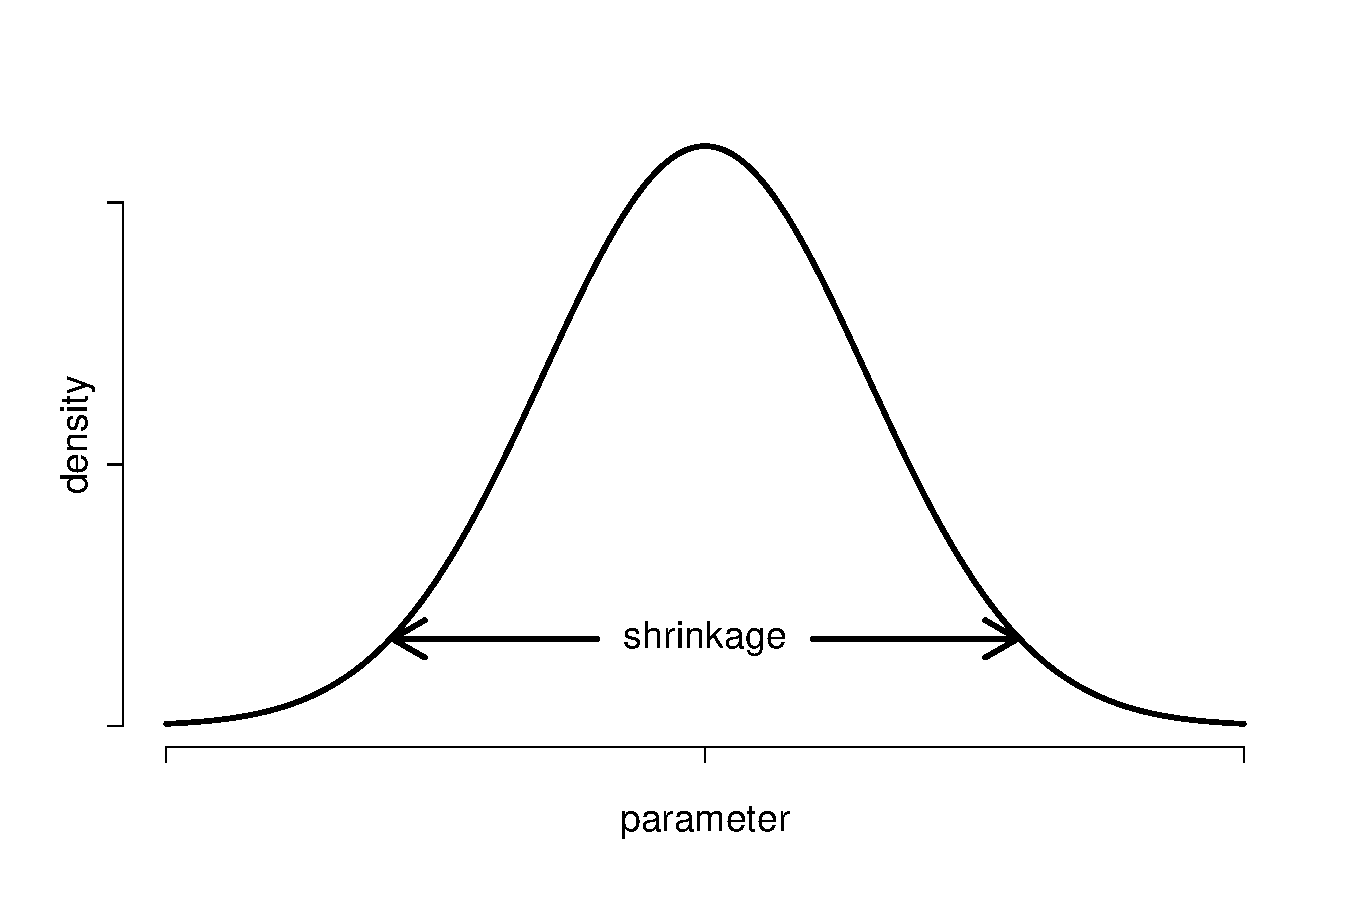
\includegraphics[scale=0.3]{shrinkage.pdf}
\end{center}

\bigskip\textbf{Prior covariance matrix.}
$$ \mathbb{V}\text{ar}[\text{vec}({\color{purple}A})] = {\color{purple}\Sigma}\otimes\underline{V} $$

\end{frame}


\begin{frame}{Minnesota prior}
\small
{\color{mcxs2}Set the column-specific prior covariance of} $A$ {\color{mcxs2}to}
\begin{align*}
\underline{V}&=\text{diag}\left(\begin{bmatrix}\kappa_2& \kappa_1\left(\mathbf{p}^{-2}\otimes\imath_N'\right)\end{bmatrix}\right)\\[2ex]
\mathbf{p} &= \begin{bmatrix} 1&2&\dots&p \end{bmatrix}\\
\imath_N &=\texttt{rep(1,N)}{\color{mcxs2}\text{ -- an $N\times1$-vector of ones}}\\
\kappa_1 &{\color{mcxs2}\text{ -- overall shrinkage level for autoregressive slopes}}\\
\kappa_2 &{\color{mcxs2}\text{ -- overall shrinkage for the constant term}}
\end{align*}

\bigskip\textbf{Prior covariance matrix.}
$$ \mathbb{V}\text{ar}[\text{vec}({\color{purple}A})] = {\color{purple}\Sigma}\otimes\underline{V} $$
\end{frame}






\begin{frame}{Minnesota prior}
\small
$$
\underline{V}=\text{diag}\left(\begin{bmatrix}\kappa_2& \kappa_1\left(\mathbf{p}^{-2}\otimes\imath_N'\right)\end{bmatrix}\right) $$

\bigskip\textbf{Stylised fact \#2.}\\
Strongly favour the unit-root hypothesis \\
{\color{mcxs2}Set prior variances for autoregressive slopes to a small number} $\kappa_1=0.02^2$

\bigskip\textbf{Stylised fact \#3.}\\
The effect of more distant lags of $y_t$ is smaller and smaller\\
{\color{mcxs2}Shrink parameters of autoregressive slopes more towards} $\underline{A}$ {\color{mcxs2}with incleasing lag} $l$ {\color{mcxs2}by dividing the corresponding prior variances by} $l^2$ {\color{mcxs2}for} $l$ {\color{mcxs2}corresponding to subsequent elements of} $\mathbf{p}$

\bigskip\textbf{Stylised fact \#4.}\\
The data are little informative about the values of $\mu_0$ \\
{\color{mcxs2}Shrink $\mu_0$ much less than autoregressive parameters} $\kappa_2\gg\kappa_1$\\ {\color{mcxs2}For instance }$\kappa_2=100$

\end{frame}





{\setbeamercolor{background canvas}{bg=mcxs2}
\begin{frame}

\begin{adjustwidth}{-0.5cm}{0cm}
%\FlushLeft
\vspace{8.3cm}\Large
\textbf{{\color{mcxs1}Posterior} {\color{mcxs5}distribution}}
\end{adjustwidth}

\end{frame}
}





\begin{frame}{Posterior distribution}

\begin{align*} 
p\left( {\color{purple}A}, {\color{purple}\Sigma}|Y,X \right) &\propto L({\color{purple}A},{\color{purple}\Sigma}|Y,X)p\left( {\color{purple}A}, {\color{purple}\Sigma} \right)\\
&= L({\color{purple}A},{\color{purple}\Sigma}|Y,X)p\left( {\color{purple}A}| {\color{purple}\Sigma} \right)p\left( {\color{purple}\Sigma} \right)
\end{align*} 

\textbf{Kernel.}
\begin{align*} 
p\left( {\color{purple}A},{\color{purple}\Sigma} |Y,X\right) 
&\propto  \text{det}({\color{purple}\Sigma})^{-\frac{T}{2}}\\
&\quad\times\exp\left\{ -\frac{1}{2}\text{tr}\left[ {\color{purple}\Sigma}^{-1}({\color{purple}A}-\widehat{A})'X'X({\color{purple}A}-\widehat{A}) \right] \right\}\\
&\quad\times \exp\left\{ -\frac{1}{2}\text{tr}\left[ {\color{purple}\Sigma}^{-1}(Y-X\widehat{A})'(Y-X\widehat{A}) \right] \right\}\\
& \quad\times\text{det}({\color{purple}\Sigma})^{-\frac{N+K+\underline{\nu}+1}{2}}\\
&\quad\times\exp\left\{ -\frac{1}{2}\text{tr}\left[ {\color{purple}\Sigma}^{-1}({\color{purple}A}-\underline{A})'\underline{V}^{-1}({\color{purple}A}-\underline{A}) \right] \right\}\\
&\quad\times \exp\left\{ -\frac{1}{2}\text{tr}\left[ {\color{purple}\Sigma}^{-1}\underline{S} \right] \right\},
\end{align*} 

\end{frame}




\begin{frame}{Posterior distribution}

\textbf{Kernel.}
\begin{align*} 
&p\left( {\color{purple}A},{\color{purple}\Sigma} |Y,X\right) \propto\text{det}({\color{purple}\Sigma})^{-\frac{T+N+K+\underline{\nu}+1}{2}}\\
&\quad\times\exp\left\{ -\frac{1}{2}\text{tr}\left[ {\color{purple}\Sigma}^{-1}\left[({\color{purple}A}-\widehat{A})'X'X({\color{purple}A}-\widehat{A}) + ({\color{purple}A}-\underline{A})'\underline{V}^{-1}({\color{purple}A}-\underline{A}) \right.\right.\right.\\
&\qquad\quad \left.\left.\left. +(Y-X\widehat{A})'(Y-X\widehat{A}) + \underline{S} \right]\right] \right\}
\end{align*} 

{\color{mcxs2}Apply the transformations and complete the squares to show that}\small
\begin{align*} 
({\color{purple}A}-\widehat{A})'&X'X({\color{purple}A}-\widehat{A}) + ({\color{purple}A}-\underline{A})'\underline{V}^{-1}({\color{purple}A}-\underline{A})  +(Y-X\widehat{A})'(Y-X\widehat{A}) + \underline{S}\\[1ex]
&= ({\color{purple}A}-\overline{A})'\overline{V}^{-1}({\color{purple}A}-\overline{A}) +
\underline{S}+Y'Y + \underline{A}'\underline{V}^{-1}\underline{A} - \overline{A}'\overline{V}^{-1}\overline{A}
\end{align*} 

\normalsize{\color{mcxs2}Now, present the kernel as the normal-inverse Wishart distribution}
\end{frame}



\begin{frame}{Joint posterior distribution}

\begin{align*} 
p\left( {\color{purple}A}, {\color{purple}\Sigma}|Y,X \right) &= p({\color{purple}A}|Y,X,{\color{purple}\Sigma})p\left( {\color{purple}\Sigma}|Y,X \right)\\[2ex]
p({\color{purple}A}|Y,X,{\color{purple}\Sigma}) &= \mathcal{MN}_{K\times N}\left( \overline{A},{\color{purple}\Sigma},\overline{V} \right)\\
p({\color{purple}\Sigma}|Y,X) &= \mathcal{IW}_N\left( \overline{S}, \overline{\nu} \right)\\[2ex]
\overline{V}&= \left( X'X + \underline{V}^{-1}\right)^{-1} \\
\overline{A}&= \overline{V}\left( X'Y + \underline{V}^{-1}\underline{A} \right)\\
\overline{\nu}&= T+\underline{\nu}\\
\overline{S}&= \underline{S}+Y'Y + \underline{A}'\underline{V}^{-1}\underline{A} - \overline{A}'\overline{V}^{-1}\overline{A}
\end{align*} 


\end{frame}







\begin{frame}{Posterior mean of $A$}

{\color{mcxs2}Posterior mean of matrix} $A$ {\color{mcxs2}is:}
\begin{align*}
\overline{A} &= {\color{mcxs2}\overline{V}}\left( X'Y + {\color{mcxs2}\underline{V}^{-1}}\underline{A} \right)\\ 
&= {\color{mcxs2}\overline{V}}\left( {\color{mcxs2}X'X}\widehat{A} + {\color{mcxs2}\underline{V}^{-1}}\underline{A} \right)\\ 
&= {\color{mcxs2}\overline{V} X'X}\widehat{A} + {\color{mcxs2}\overline{V}\underline{V}^{-1}}\underline{A} 
\end{align*}
{\color{mcxs2}a linear combination of the MLE} $\widehat{A}$ {\color{mcxs2}and the prior mean} $\underline{A}$

\end{frame}


{\setbeamercolor{background canvas}{bg=mcxs2}
\begin{frame}{\color{mcxs1}Bayesian VARs}
\begin{description}
\item[Bayesian VARs] {\color{mcxs5}are benchmark models for macroeconomic forecasting}

\smallskip\item[Closed-form] {\color{mcxs5}solutions to the estimation problem allow fast computations}

\smallskip\item[Minnesota prior] {\color{mcxs5}reflects stylized facts about macroeconomic time series}

\smallskip\item[Large Bayesian VARs] {\color{mcxs5}use the Kronecker structure of covariance matrix and the application of shrinkage for precise economic forecasting}
\end{description}
\end{frame}
}

\end{document} 